%!TEX root = ../DissertationDefensePresentation.tex

%%--------------------------------------------------------------------------------------------

\subsection*{MC Corrections}

%%--------------------------------------------------------------------------------------------

\begin{frame}
	\frametitle{MC Corrections}
	\framesubtitle{Pileup Reweighting}
	\vspace*{-0.24cm}
	\begin{block}{}
		\begin{itemize}
			\small
			\item MC samples generated using the 2012 assumed pileup scenario
			\item The number of true pileup interactions ($\mu$) is reweighted to match the distribution expected in data
		\end{itemize}
	\end{block}
	\begin{figure}
		\centering
		\begin{subfigure}[t]{0.32\textwidth}
			\includegraphics[width=\textwidth]{\anpath/dataPUdist.png}
		\end{subfigure}
		\begin{subfigure}[t]{0.32\textwidth}
			\includegraphics[width=\textwidth]{\anpath/MCPUdist.png}
		\end{subfigure}
		\begin{subfigure}[t]{0.32\textwidth}
			\includegraphics[width=\textwidth]{\anpath/Weights.png}
		\end{subfigure}
	\end{figure}
	\begin{textblock}{0.2}(0.32,0.50){\color{red}$\div$}\end{textblock}
	\begin{textblock}{0.2}(0.645,0.50){\color{blue}$=$}\end{textblock}
	\vspace*{-0.30cm}
	\begin{figure}
		\centering
		\begin{subfigure}[t]{0.32\textwidth}
			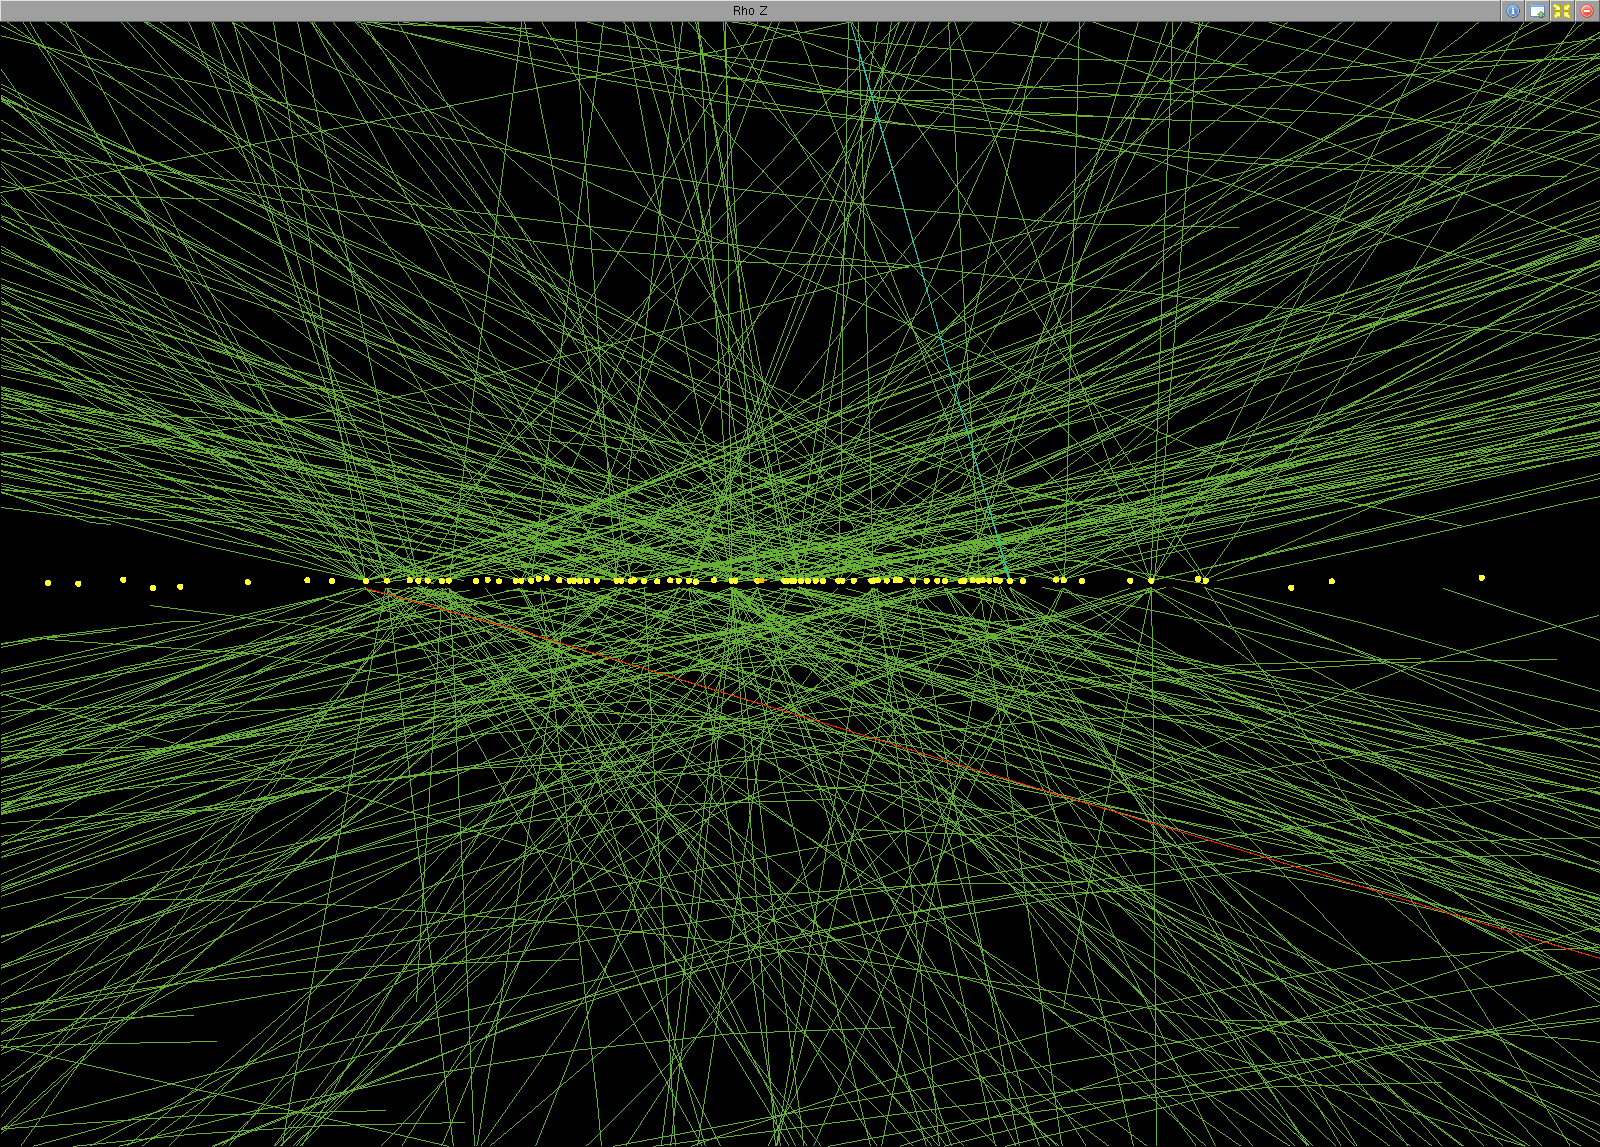
\includegraphics[width=\textwidth]{\figpath/vertices.png}
		\end{subfigure}
		\begin{subfigure}[t]{0.32\textwidth}
			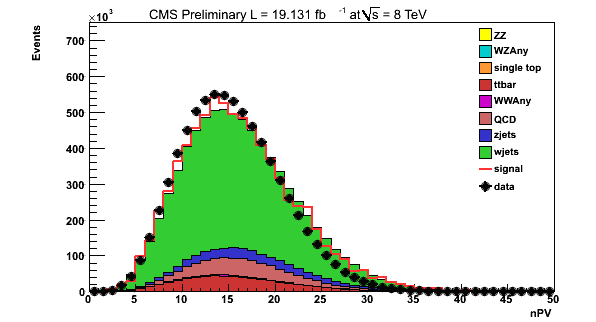
\includegraphics[width=\textwidth]{\figpath/nPV_noRW__comblep_trim.png}
		\end{subfigure}
		\begin{subfigure}[t]{0.32\textwidth}
			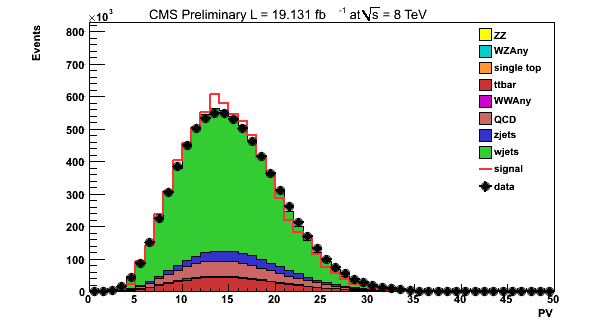
\includegraphics[width=\textwidth]{\figpath/nPV__comblep_trim.png}
		\end{subfigure}
	\end{figure}
	\begin{textblock}{0.2}(0.655,0.85){\color{Orange}$\Rightarrow$}\end{textblock}
	\begin{textblock}{0.35}(0.46,0.69){\color{Orange}\Large{Before}}\end{textblock}
	\begin{textblock}{0.35}(0.79,0.69){\color{Orange}\Large{After}}\end{textblock}
\end{frame}

\begin{frame}
	\frametitle{MC Corrections}
    \framesubtitle{Jet Corrections}
    \vspace*{-0.24cm}
    \begin{block}{Jet Energy Corrections}
    	\begin{itemize}
	    	\footnotesize
    		\item Corrects the scale of jets due to pileup and detector effects
    		\item L1FastJet (pileup), L2Relative ($\eta$ dependent), and L3Absolute ($p_{T}$ dependent) corrections
    		\item L2L3Residual (MC/data) corrections used on data only
    	\end{itemize}
    \end{block}
    \vspace*{1.4cm}
    \begin{block}{Jet Energy Resolution}
    	\begin{itemize}
    		\footnotesize
    		\item Deterministic $\eta$-dependent corrections for jets and $\Em_{T}$
    		\item Multiplicative correction factor follows the form shown below
    	\end{itemize}
    \end{block}
    \vspace*{-0.50cm}
    \begin{columns}[T]
    	\begin{column}{0.27\textwidth}
    		\begin{block}{JER Constants}
    			\tiny
    			\begin{table}[ht]
					\centering
					\begin{tabular}{| l | l |}
						\hline\hline\\[-2.75ex]
						$\eta$ &JER Correction\\
						\hline\\[-2.75ex]
						$<0.5$ & $1.052$\\
						\hline\\[-2.75ex]
						$\geqslant0.5\&<1.1$ & $1.057$\\
						\hline\\[-2.75ex]
						$\geqslant1.1\&<1.7$ & $1.096$\\
						\hline\\[-2.75ex]
						$\geqslant1.7\&<2.3$ & $1.134$\\
						\hline\\[-2.75ex]
						$\geqslant2.3\&<5.0$ & $1.288$\\
						\hline\hline
					\end{tabular}
					\label{tab:jer}
					\vspace*{-0.3cm}
				\end{table}
			\end{block}
    	\end{column}
    	\begin{column}{0.32\textwidth}
    		\begin{block}{JER Correction}
    			\Tiny
    			\begin{equation}
				\label{eq:C_JER}
				C_{JER}=max\left(0.0,\frac{p_{T}^{GEN}}{p_{T}^{RECO}}+C_{\eta}\cdot\left(1-\frac{p_{T}^{GEN}}{p_{T}^{RECO}}\right)\right)
				\end{equation}
				\begin{equation}
				\label{eq:Jet_JER}
				Jet_{\textbf{X}}^{corrected}=C_{JER}{\cdot}Jet_{\textbf{X}}^{RECO}
				\end{equation}
    		\end{block}
    	\end{column}
    	\begin{column}{0.34\textwidth}
    		\begin{block}{Propogate to $\Em_{T}$}
    			\tiny
    			\begin{equation}
				\Em_{x}^{corrected}=\left(1-C_{JER}\right)Jet_{x}^{RECO}+{\Em_{T}}_{x}^{RECO}\label{eq:MET_JER_X}
				\end{equation}
				\begin{equation}
				\Em_{y}^{corrected}=\left(1-C_{JER}\right)Jet_{y}^{RECO}+{\Em_{T}}_{y}^{RECO}\label{eq:MET_JER_Y}
				\end{equation}
    		\end{block}
    	\end{column}
    \end{columns}
	\begin{textblock}{1.0}(0.07,0.325)
		\begin{figure}
			\centering
			\scalebox{0.6}{\input{JEC_levels}}
			\label{fig:factorized_approach}
		\end{figure}
	\end{textblock}
\end{frame}

\begin{frame}%<1>[label=frame:event_selection_met_phi]
	\frametitle{MC Corrections}
	\framesubtitle{$\Em_{\phi}$ Reweighting}
	\vspace*{-0.54cm}
	\begin{columns}[T]
		\begin{column}{0.52\textwidth}
			\begin{block}{}
				\begin{itemize}
					\item Clear modulation in the $\Em_{\phi}$ distributions for both data and MC
					\item In 2012 this was peramterized in terms of NPV
					\item $\Em_{\phi}$ correction follows the equations below
				\end{itemize}
%				\vspace*{-0.15cm}
				\begin{equation}
				\Em_{x}^{corrected}=\Em_{x}^{RECO}-\left([0]+[1]{\cdot}nPV\right)\label{eq:METPhi_cor_x}
				\end{equation}
				\begin{equation}
				\Em_{y}^{corrected}=\Em_{y}^{RECO}-\left([0]+[1]{\cdot}nPV\right)\label{eq:METPhi_cor_y}
				\end{equation}
				\vspace*{-0.55cm}
				\begin{table}[hbtp]\footnotesize
					\centering
					\begin{tabular}{|c|c|l|}
					\hline\hline
					Sample & Parameter 0 & Parameter 1 \\
					\hline
					\textbf{Data} & & \\
					x & $2.0105E-01$ & $4.2663E-01$ \\
					\hline
					y & $-9.1350E-01$ & $-2.3120E-01$ \\
					\hline\hline
					\textbf{MC} & & \\
					x & $2.9059E-01$ & $-3.5293E-03$ \\
					\hline
					y & $3.0183E-01$ & $-1.9974E-01$ \\
					\hline\hline
					\end{tabular}
					\label{tab:METPhi_cor_xy}
				\end{table}
			\end{block}
		\end{column}
		\begin{column}{0.45\textwidth}
			\begin{figure}
				\centering
				\begin{subfigure}[t]{\textwidth}
					\only<1>{\includegraphics[width=\textwidth]{\anpath/METPhi_Before-eps-converted-to.pdf}}
					\only<2>{\includegraphics[width=\textwidth]{\anpath/METPhi_After-eps-converted-to.pdf}}
				\end{subfigure}
				\newline
				\begin{subfigure}[t]{\textwidth}
					\only<1>{\includegraphics[width=\textwidth]{\anpath/METxyVsNPV_Before-eps-converted-to.pdf}}
					\only<2>{\includegraphics[width=\textwidth]{\anpath/METxyVsNPV_After-eps-converted-to.pdf}}
				\end{subfigure}
			\end{figure}
		\end{column}
	\end{columns}
\end{frame}
%\againframe<2>{frame:event_selection_met_phi}

\begin{frame}
	\frametitle{MC Corrections}
	\framesubtitle{$p_{T}^{Top}$ Reweighting}
	\vspace*{-0.34cm}
	\begin{columns}[T]
		\begin{column}{0.5\textwidth}
			\begin{block}{}
				\begin{itemize}
					\item The top quark $p_{T}$ spectrum in data is softer than found in the NNLO predictions
					\item Right: Fit of $p_{T}^{Top}$ for data/MC in multiple analysis regimes
					\item Top weights were derived as a function of the generated $p_{T}$ of the top quark pair
					\begin{itemize}
						\item Correction only applied to TTbar sample where there exists a top quark pair
					\end{itemize}
				\end{itemize}
				\begin{equation}\label{eq:ttbar_weight_1}
				Weight=\sqrt{SF\left(t\right)SF\left(\bar{t}\right)}
				\end{equation}
				\begin{equation}\label{eq:ttbar_weight_2}
				SF\left(x\right)=e^{a+b{\cdot}x}
				\end{equation}
				\begin{equation}\label{eq:ttbar_weight_2}
				x=p_{T}\text{, }a=0.159\text{, }b=-0.00141
				\end{equation}
			\end{block}
		\end{column}
		\begin{column}{0.46\textwidth}
			\vspace*{0.5cm}
			\begin{figure}
				\centering
				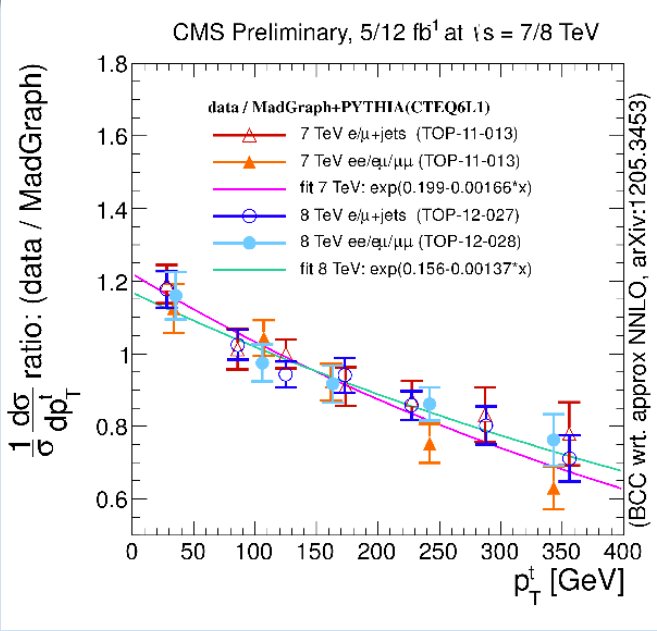
\includegraphics[width=\textwidth]{\figpath/TopPt_Data_MC}
			\end{figure}
		\end{column}
	\end{columns}

\end{frame}

%%--------------------------------------------------------------------------------------------

\subsection*{QCD Model}

%%--------------------------------------------------------------------------------------------
\begin{frame}
	\frametitle{Data-Driven QCD Model}
	\vspace*{-0.24cm}
	\begin{block}{}
		\begin{itemize}
			\small
			\item The QCD multijet background:
			\begin{itemize}
				\footnotesize
				\item Hard to model because of the non-perturbative nature of QCD
				\item Few MC events pass our selection criteria even though the MC samples are large
			\end{itemize}
			\item Data-driven technique:
			\begin{itemize}
				\footnotesize
				\item Make use of the full 2012 single lepton datasets (same datasets mentioned before)
				\item Selection criteria ensures that the events are orthogonal to the data selection
			\end{itemize}
		\end{itemize}
	\end{block}
	\vspace*{-0.49cm}
	\begin{columns}[T]
		\column{0.48\textwidth}
			\vspace*{-0.1cm}
			\begin{center}
				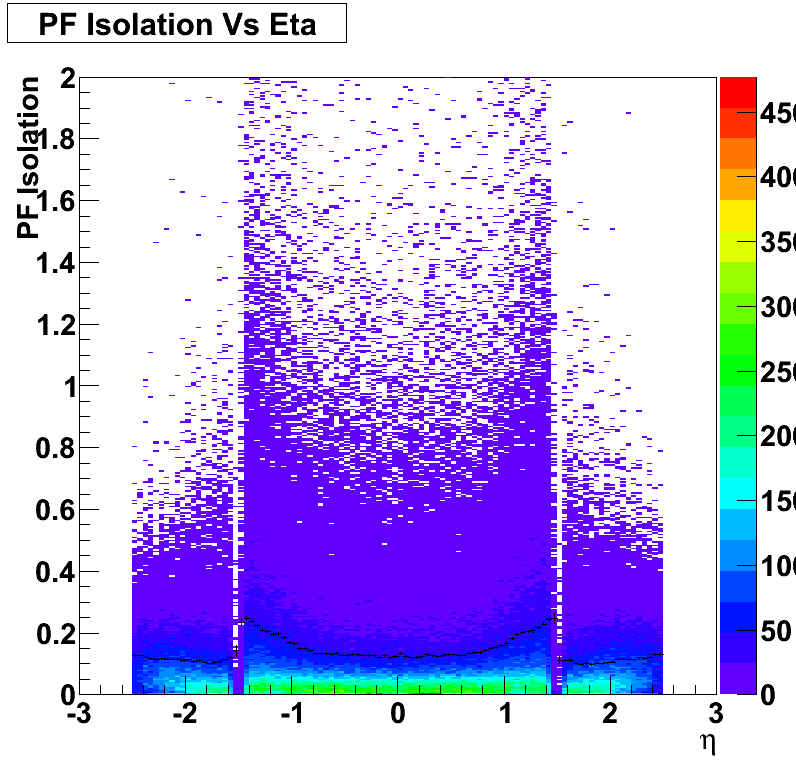
\includegraphics[width=0.9\textwidth]{\figpath/pfIsoVsEta_Full.png}
			\end{center}
		\column{0.49\textwidth}
			\begin{block}{Selection Criteria}
				\begin{itemize}
					\scriptsize
					\item Our QCD sample is obtained from the anti-isolated lepton region (antiIso)
					\vspace*{-0.15cm}
					\item Electrons:
					\begin{itemize}
						\scriptsize
						\item Drop MVA ID requirement
						\item PF Isolation: $<0.2{\rightarrow}>0.3$
					\end{itemize}
					\vspace*{-0.25cm}
					\item Muons:
					\begin{itemize}
						\scriptsize
						\item PF Isolation: $<0.12{\rightarrow}>0.2$
					\end{itemize}
				\end{itemize}
			\end{block}
			\vspace*{-0.30cm}
			\begin{block}{}
				\begin{enumerate}
					\scriptsize
					\item Must PU reweight as $N_{PV}$ distribution different in antiIso region than in SR (selection bias)
					\vspace*{-0.1cm}
					\item Ratio of events in signal region to anti-isolated region varies as a function of $\eta$ (studied in MC)
					\begin{itemize}
						\scriptsize
						\item Transform expected yields to match SR by fitting the $\Em_{T}$ distributions of QCD and \Wjets to data
					\end{itemize}
				\end{enumerate}
			\end{block}
	\end{columns}

	\begin{textblock}{0.5}(0.01,0.93)
		\scriptsize 1.09\% contamination from non-QCD events
	\end{textblock}
\end{frame}

\begin{frame}
	\frametitle{Data-Driven QCD Model}
	\framesubtitle{Methodology}
	\vspace*{-0.24cm}
	\begin{columns}[T]
		\begin{column}{0.49\textwidth}
			\vspace*{-0.3cm}
			\begin{block}{Shape}
				\vspace*{-0.35cm}
				\begin{aeq}{eq:N_QCD_sig}
					N_{SR}^{QCD}\left(\eta\right)=N_{antiIso}^{QCD}\left(\eta\right){\cdot}s^{QCD}\left(\eta\right)
				\end{aeq}
				\vspace*{-0.35cm}
				\begin{itemize}
					\footnotesize
					\item $N_{antiIso}^{QCD}$ and $N_{SR}^{QCD}$ are the number of QCD events in the antiIso and SR for a given luminosity
					\item $s^{QCD}$: transfer weight obtained from fit{\tikz[remember picture]{\node[coordinate] (s-fit) {};}}
					\item \Wjets (biggest background) and QCD have differently shaped $\Em_{T}$ distributions
				\end{itemize}
			\end{block}
			\vspace*{-0.25cm}
			\begin{block}{Normalization over all $\eta$}
				\begin{itemize}
					\footnotesize
					\item Determine the QCD \& \Wjets event yields (global scale factor):
					\begin{itemize}
						\footnotesize
						\item Fit to the $\Em_{T}$ distribution with all $\eta$ bins combined
						\item Done in the $\geqslant2$ jets bin
						\item The fit gives us the QCD normalization and a scale factor for \Wjets (very close to 1)
					\end{itemize}
				\end{itemize}
			\end{block}
		\end{column}
		\begin{column}{0.48\textwidth}
			\begin{tikzpicture}[remember picture]
				\node [inner sep=0pt,above right] {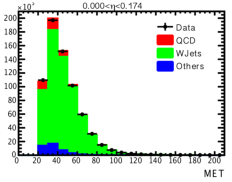
\includegraphics[width=\textwidth]{\figpath/SingleMetFit_control6_electron_crop.pdf}};
				\node[anchor=base] (fit) at (1.2,3) {};
			\end{tikzpicture}
			\begin{table}[ht]
				\caption{\scriptsize{Absolute scale factors for the \Wjets and QCD samples in the electron and muon channels}}
				\centering
				\scriptsize
				\begin{tabular}{| l | c | r |}
					\hline\hline\\[-2.7ex]
					& Electrons & Muons\\
					\hline\\[-2.7ex]
					WJets & $1.045\pm0.005$ & $0.970\pm0.004$\\
					\hline\\[-2.7ex]
					QCD & $0.249\pm0.013$ & $0.145\pm0.007$\\
					\hline
				\end{tabular}
				\label{tab:yields}
			\end{table}
		\end{column}
	\end{columns}
	\begin{textblock}{0.25}(0.83,0.38)
		1 jet CR
	\end{textblock}
	\begin{textblock}{0.25}(0.70,0.25)
		\color{red} Floating
	\end{textblock}
	\begin{textblock}{0.25}(0.70,0.285)
		\color{green} Floating
	\end{textblock}
	\begin{textblock}{0.25}(0.70,0.32)
		\color{blue} Fixed
	\end{textblock}
	\begin{tikzpicture}[overlay]
			\path[->,violet,thick] ([xshift=1mm,yshift=1mm]s-fit) edge [out=0,in=180] (fit);
	\end{tikzpicture}
\end{frame}

\begin{frame}<1>[label=frame:qcd_model_normalization]
	\frametitle{Data-Driven QCD Model}
	\framesubtitle{Final Product}
	\vspace*{-0.24cm}
		\begin{textblock}{0.50}(0.25,0.12)
			\begin{center}
				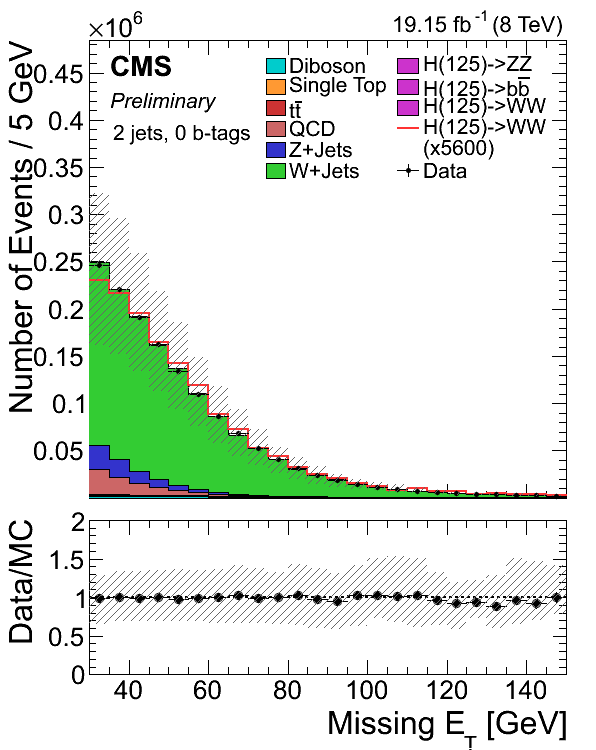
\includegraphics[width=0.95\textwidth]{\figpath/MET_electron.png}
			\end{center}
		\end{textblock}
		\begin{textblock}{0.50}(0.45,0.40)
			{\color{orange}\Large Excellent\\Agreement!}
		\end{textblock}
\end{frame}

%%--------------------------------------------------------------------------------------------

\subsection*{Validation}

%%--------------------------------------------------------------------------------------------

\begin{frame}
	\frametitle{Kinematic Validation Plots}
	\framesubtitle{2 Jets - Muon Bin}
	\begin{block}{}
		\begin{itemize}
			\item Some relevant distributions shown here
			\begin{itemize}
			 	\item Good agreement in all distributions
			 	\item Similar agreement for muons and other jet bins 
			 \end{itemize}
		\end{itemize}
	\end{block}
	\vspace*{-0.24cm}
	\begin{columns}[T]
		\column{0.31\textwidth}
			\begin{block}{\scriptsize \Mjj}
				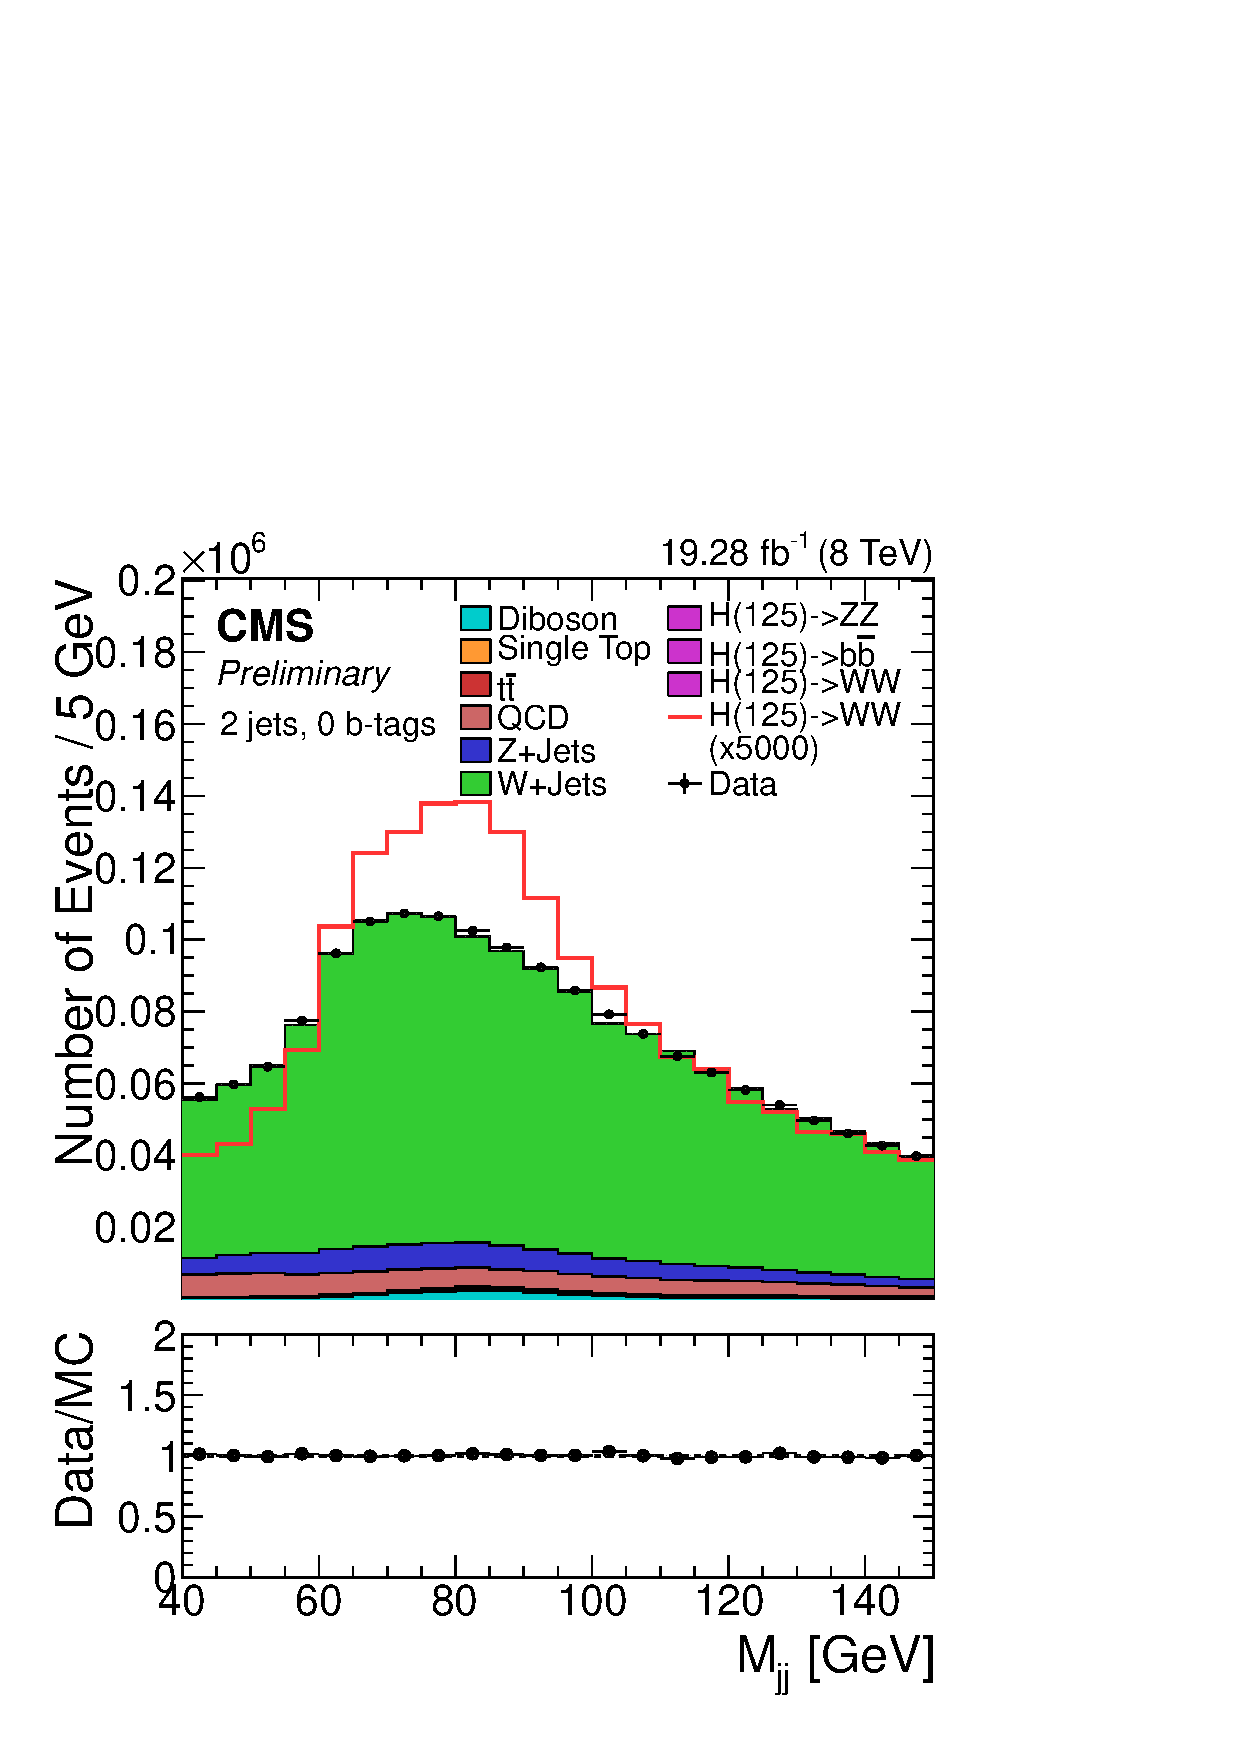
\includegraphics[width=\textwidth]{\figpath/Mjj_muon_2jets.pdf}%
			\end{block}
		\column{0.31\textwidth}
			\begin{block}{\scriptsize \Mlv}
				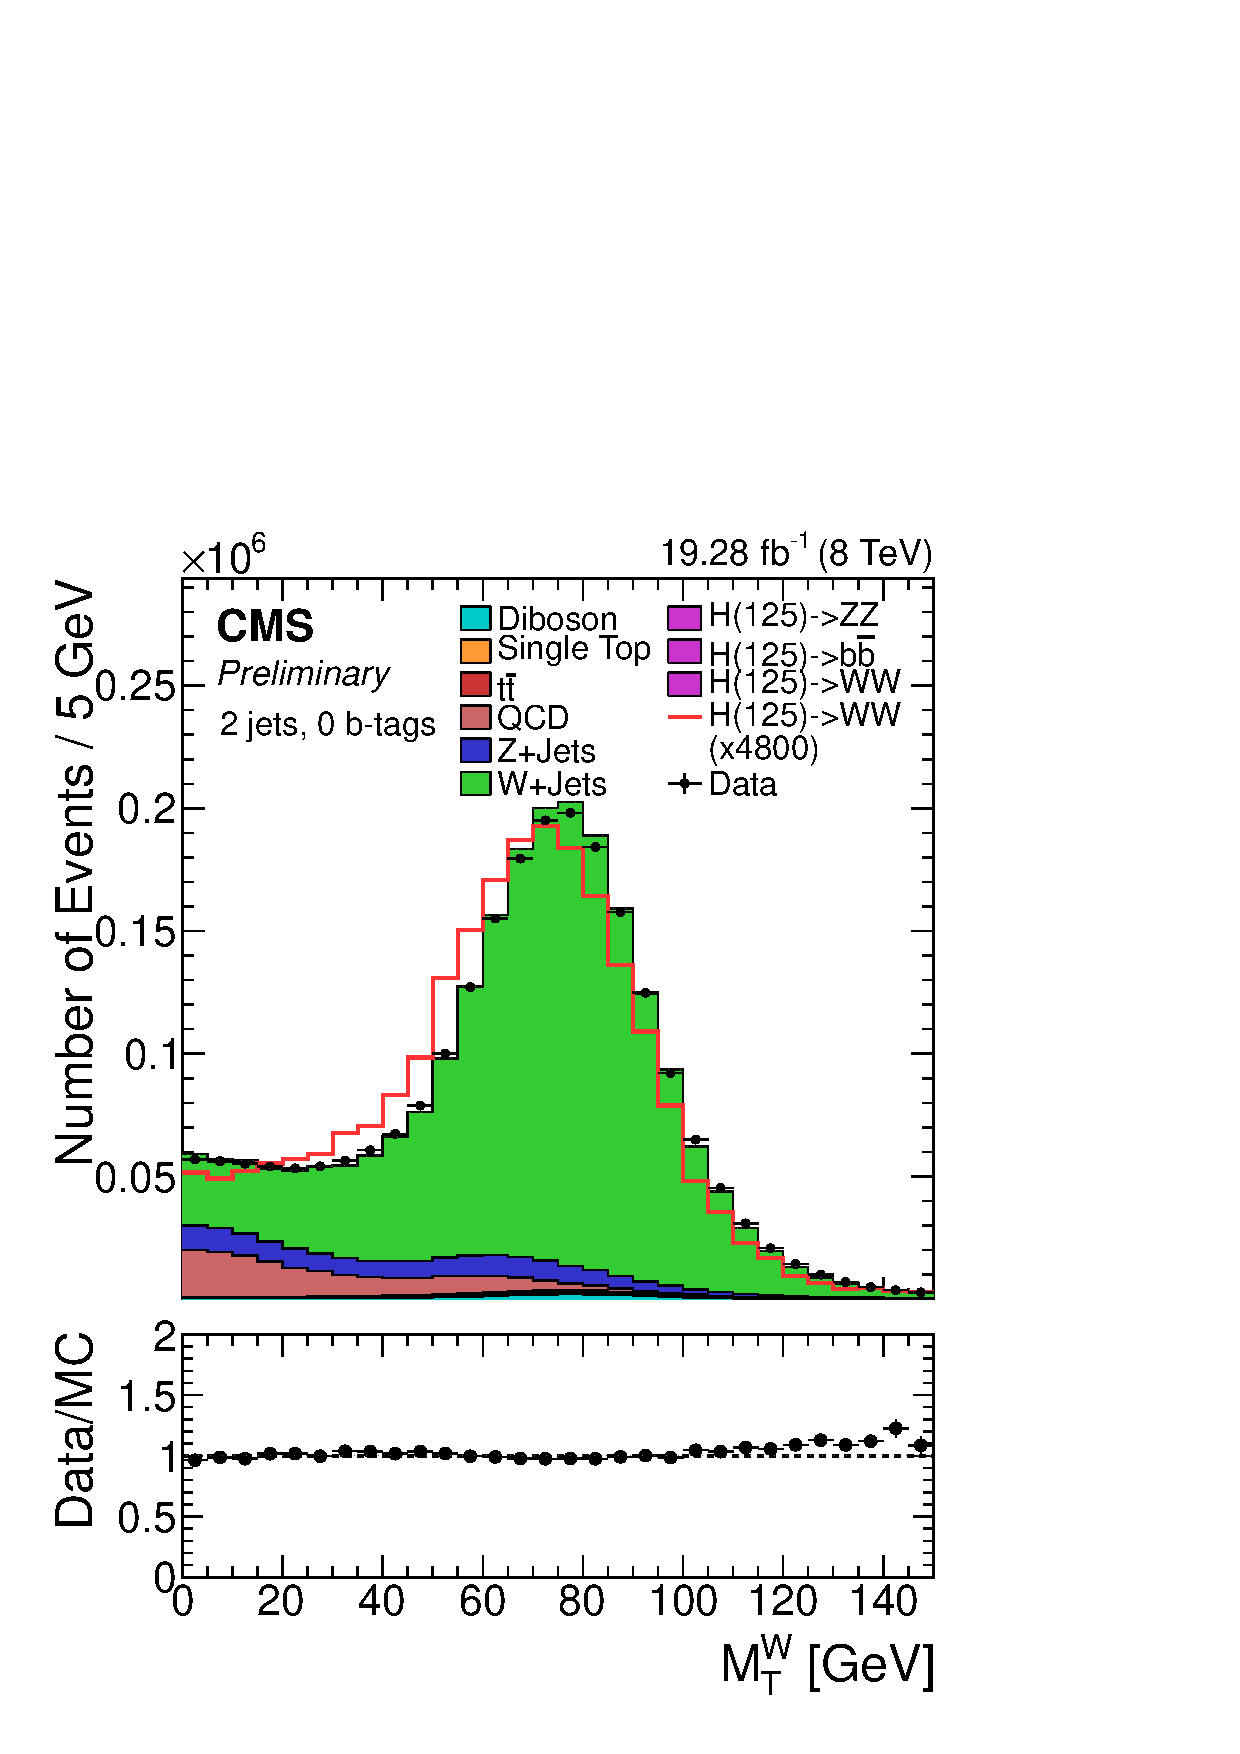
\includegraphics[width=\textwidth]{\figpath/WmT_muon_2jets.pdf}%
			\end{block}
		\column{0.31\textwidth}
			\begin{block}{\scriptsize \Mlvjj}
				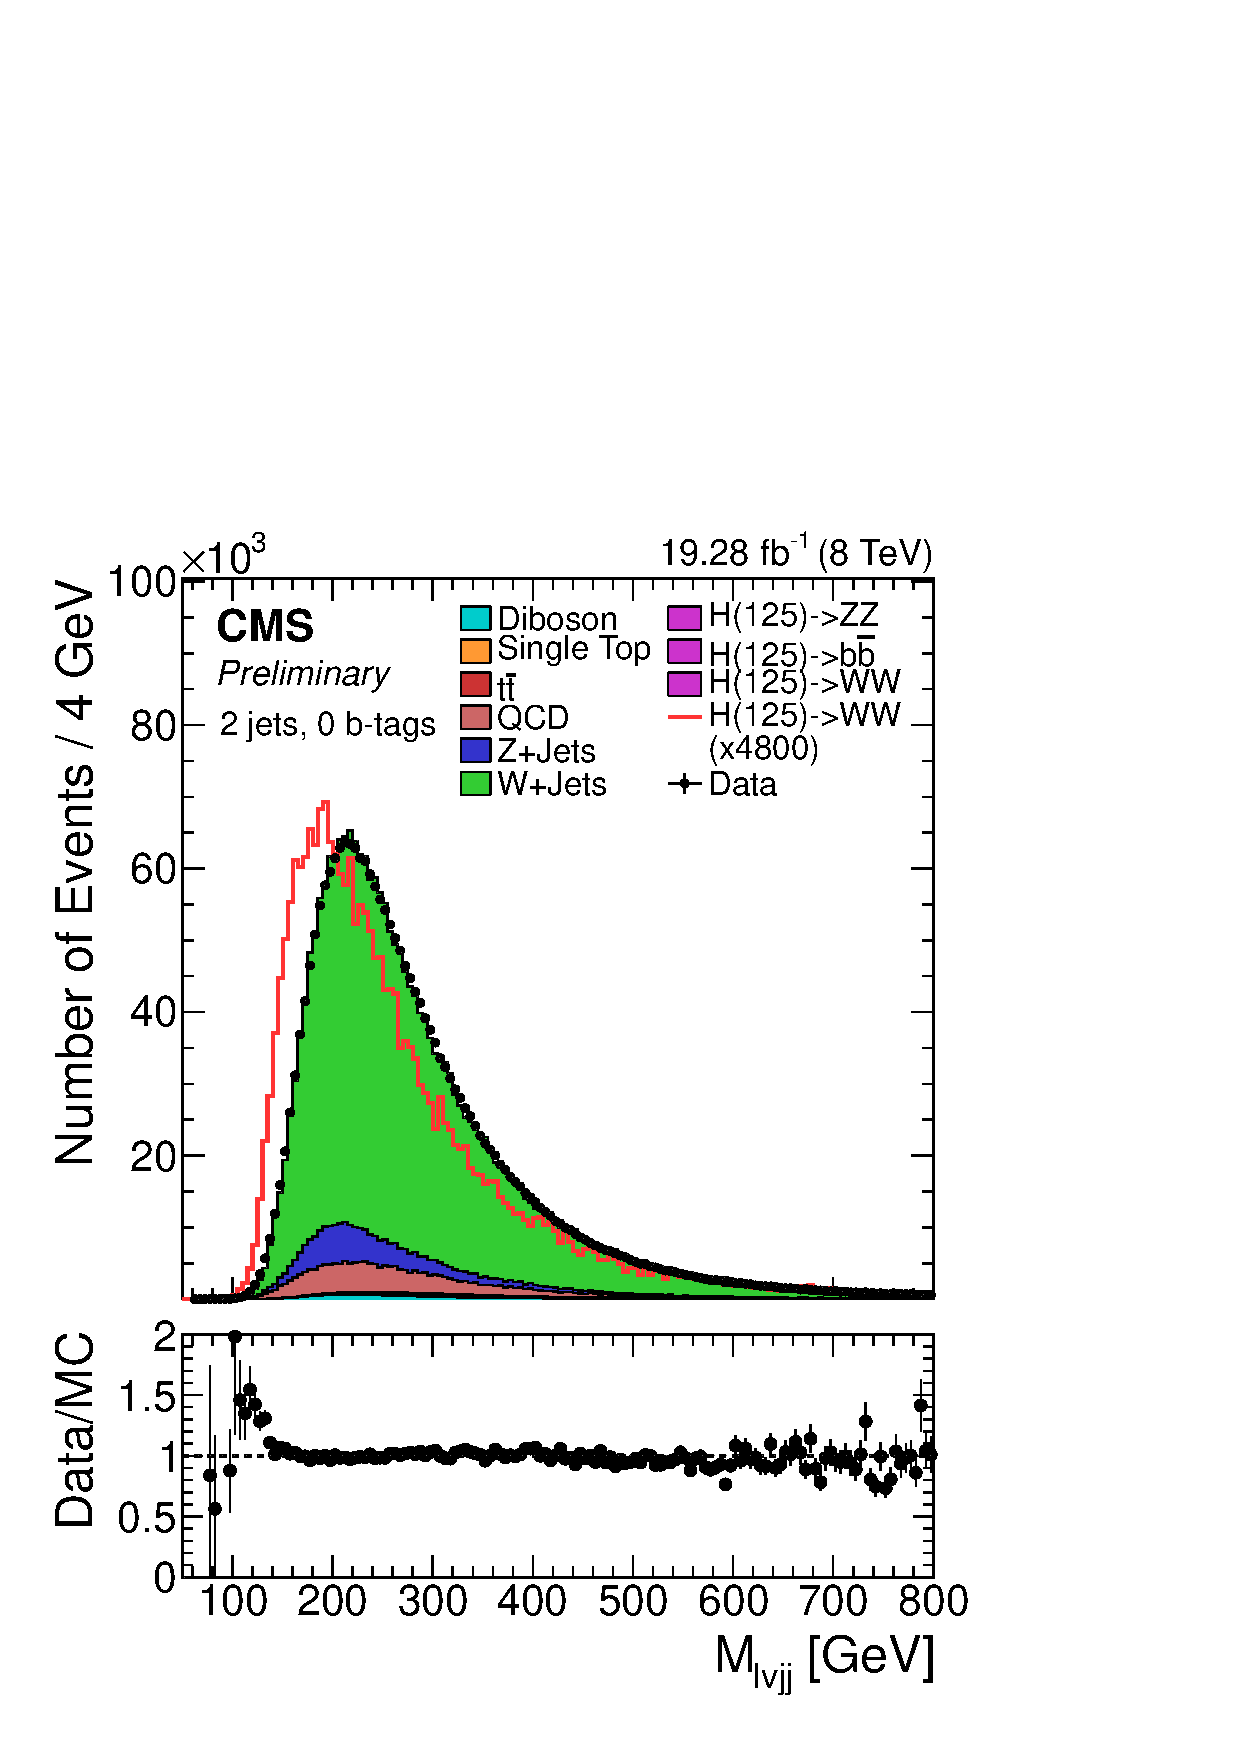
\includegraphics[width=\textwidth]{\figpath/Mlvjj_muon_2jets.pdf}%
			\end{block}
	\end{columns}
\end{frame}

%%--------------------------------------------------------------------------------------------

\subsection*{Yields}

%%--------------------------------------------------------------------------------------------

\begin{frame}
	\frametitle{Expected Yields}
	\begin{itemize}
		\item Table of expected yields split by jet category (2, 3, or $\geqslant$4) for the combined lepton category ($\Pe+\Pmu$)
	\end{itemize}
	\begin{table}[htbp]
		\color{black}
		\centering
		\scriptsize
		\label{tab:NoBTagYield}
		\begin{tabular}{|p{3.5cm}|c|c|c|} \hline
			\textbf{Process} & \textbf{2 Jets} & \textbf{3 Jets} & \textbf{$\geqslant$4 Jets}\\ \hline
			Diboson & $46495.97\pm78.55$ & $15049.18\pm44.70$ & $4150.48\pm23.47$ \\
			\rowonly<2>{\rowcolor{ForestGreen}}
			\Wjets & $3446003.06\pm6434.30$ & $756463.35\pm3008.63$ & $189815.29\pm1515.40$ \\
			\Zjets & $270460.62\pm822.24$ & $69061.73\pm415.90$ & $19829.24\pm222.71$ \\
			\ttbar & $22452.06\pm142.85$ & $27902.44\pm160.86$ & $31218.33\pm170.54$ \\
			Single \cPqt & $16587.13\pm84.31$ & $7193.89\pm59.29$ & $3068.60\pm40.25$ \\
			Multijet & $275465.33\pm952.52$ & $74168.89\pm504.39$ & $22109.53\pm282.94$ \\\hline
			\rowtemporal<2>{\rowcolor{mygray}}{\rowcolor{ForestGreen}}{\rowcolor{mygray}}
			Total Background & $4077464.17\pm6558.75$ & $949839.48\pm3083.93$ & $270191.47\pm1567.59$ \\\hline
			\ggH, \HWW \MH=125\gev & $552.09\pm1.92$ & $211.15\pm1.19$ & $79.51\pm0.73$ \\
			\qqH, \HWW \MH=125\gev & $106.60\pm0.56$ & $52.66\pm0.39$ & $17.51\pm0.23$ \\
			\WH\_\ZH\_\ttH \newline \HWW \MH=125\gev & $136.20\pm2.22$ & $84.35\pm1.75$ & $42.32\pm1.22$ \\\hline
			\rowtemporal<3>{\rowcolor{mygray}}{\rowcolor{Mulberry}}{\rowcolor{mygray}}
			Total \HWW & $794.89\pm2.99$ & $348.16\pm2.15$ & $139.34\pm1.44$ \\\hline
			\WH\_\ZH\_\ttH \newline \HZZ \MH=125\gev & $10.30\pm0.17$ & $5.30\pm0.12$ & $2.35\pm0.08$ \\
			\WH, \Hbb \MH=125\gev & $45.34\pm0.40$ & $14.22\pm0.23$ & $3.86\pm0.12$ \\
			\ttH, \Hbb \MH=125\gev & $0.59\pm0.03$ & $1.33\pm0.05$ & $3.77\pm0.09$ \\\hline
			\rowcolor{mygray}
			Total Volunteer Signal & $56.23\pm0.44$ & $20.85\pm0.26$ & $9.98\pm0.17$ \\\hline
			\rowonly<4>{\rowcolor{red}}
			Signal \textsubscript{\HWW}/Bkg & 0.000195 & 0.000367 & 0.000516 \\
			Signal \textsubscript{\HWW}/$\sqrt{\text{Bkg}}$ & 0.394 & 0.357 & 0.268 \\\hline
			\rowcolor{mygray}
			Data & $4057594$ & $953513$ & $272713$ \tabularnewline\hline
		\end{tabular}
	\end{table}
	\begin{itemize}
		\item \only<4>{\color{red}}The background is $\sim5000$ times bigger than the signal
	\end{itemize}
\end{frame}